
\documentclass[
11pt, % Set the default font size, options include: 8pt, 9pt, 10pt, 11pt, 12pt, 14pt, 17pt, 20pt
%t, % Uncomment to vertically align all slide content to the top of the slide, rather than the default centered
%aspectratio=169, % Uncomment to set the aspect ratio to a 16:9 ratio which matches the aspect ratio of 1080p and 4K screens and projectors
]{beamer}

\graphicspath{{Images/}{./}} % Specifies where to look for included images (trailing slash required)

\usepackage{todonotes}
\usepackage{graphicx}
\usepackage{xcolor}
\usepackage{subfig}
%%\usepackage[noend]{algpseudocode}


\usepackage{algorithm}
\usepackage{algorithmic}

\usepackage{blkarray}
\usepackage{amsmath}
\usepackage{xspace}
\usepackage{float}


\usepackage{tikz}
\usetikzlibrary{matrix, decorations, patterns, positioning, shapes, calc, intersections, arrows, fit}

\usetikzlibrary{patterns}
\usetikzlibrary{fit,calc,positioning,decorations.pathreplacing,matrix}

\usepackage{booktabs} % Allows the use of \toprule, \midrule and \bottomrule for better rules in tables


\newcommand{\brown}[1]{{\color{brown} #1 }}

%% Colors from https://latexcolor.com/
\definecolor{pastelviolet}{rgb}{0.8, 0.6, 0.79}
\definecolor{babyblueeyes}{rgb}{0.63, 0.79, 0.95}
\definecolor{pastelyellow}{rgb}{0.99, 0.99, 0.59}
\definecolor{pastelgreen}{rgb}{0.47, 0.87, 0.47}
\definecolor{pastelred}{rgb}{1.0, 0.41, 0.38}
\colorlet{patternblue}{blue!60}

\usetheme{Madrid}





%----------------------------------------------------------------------------------------
%	PRESENTATION INFORMATION
%----------------------------------------------------------------------------------------

\title[Matrix multiplication]{Communication costs of sequential matrix multiplications} % The short title in the optional parameter appears at the bottom of every slide, the full title in the main parameter is only on the title page

%\subtitle{Optional Subtitle} % Presentation subtitle, remove this command if a subtitle isn't required

\author[Suraj Kumar]{Suraj Kumar} % Presenter name(s), the optional parameter can contain a shortened version to appear on the bottom of every slide, while the main parameter will appear on the title slide

\institute[Inria \& ENS Lyon]{Inria \& ENS Lyon \\ \smallskip Email:\textit{suraj.kumar@inria.fr}} % Your institution, the optional parameter can be used for the institution shorthand and will appear on the bottom of every slide after author names, while the required parameter is used on the title slide and can include your email address or additional information on separate lines

\date[CR12]{CR12: September 2023\\ \smallskip\small https://surakuma.github.io/courses/daamtc.html} % Presentation date or conference/meeting name, the optional parameter can contain a shortened version to appear on the bottom of every slide, while the required parameter value is output to the title slide

%----------------------------------------------------------------------------------------

\begin{document}
	
	%----------------------------------------------------------------------------------------
	%	TITLE SLIDE
	%----------------------------------------------------------------------------------------
	
	\begin{frame}
		\titlepage % Output the title slide, automatically created using the text entered in the PRESENTATION INFORMATION block above
	\end{frame}

	


\section{Matrix multiplication}
	\begin{frame}{Table of Contents}		
	\tableofcontents[currentsection,hideallsubsections] % Output the table of contents (all sections on one slide)		
\end{frame}

\begin{frame}{Traditional matrix multiplication}
	\begin{itemize}
		\item $C= AB$, where $A \in\mathbb{R}^{m \times k}$, $B \in\mathbb{R}^{k \times n}$, and  $C$ $\in$ $\mathbb{R}^{m \times n}$.
		\item $C_{ij} = \sum_p A_{ip}*B_{pj}$
	\end{itemize}
	For simplicity, we assume $m=k=n$ throughout the presentation.
	\begin{center}
		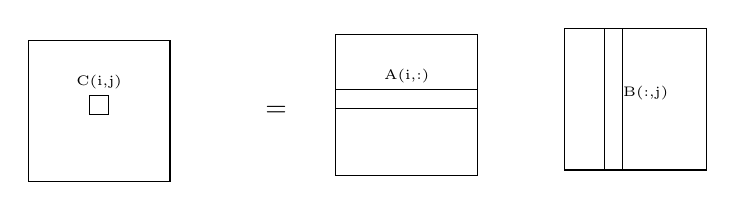
\begin{tikzpicture}[scale=1, every node/.style={transform shape}]
		%%	\tikzstyle{taskr}=[draw=black, minimum height=18mm, minimum width=18mm, anchor=south west, fill=pastelgreen, text=black]
		
		\tikzstyle{taskr}=[draw=black, minimum height=18mm, minimum width=18mm, fill=pastelgreen, text=black]
		
		\tikzstyle{taskrow}=[draw=black, minimum height=2mm, minimum width=18mm, fill=pastelgreen, fill=none, text=black]
		\tikzstyle{taskcol}=[draw=black, minimum height=18mm, minimum width=2mm, fill=pastelgreen, fill=none, text=black]
		
		\tikzstyle{taskrsmall}=[draw=black, minimum height=2mm, minimum width=2mm, fill=none, text=black]
		
		%%	\node(t1) at (0,0) {};
		%%	\node [above right=0cm and 0cm of t1.mid,taskr](T1) {};
		\node [taskr, fill=none] (T1) at (0,0) {};
		\node [taskrsmall] (T2) at (T1.mid) {};
		\node [above] at (T2.mid) {\tiny C(i,j)};
		\node[draw=none, text=black, scale=1] at (2.25,0) {$=$};
		
		\node [right=3cm of T1.mid,taskr, fill=none](T3) {};
		\node[taskrow](T4) at (T3.mid) {};
		\node [above] at (T4.mid) {\tiny A(i,:)};
		
		\node [right=2cm of T3.mid,taskr, fill=none](T5) {};
		\node [right=2.5cm of T3.mid, taskcol](T6) {};
		\node [right] at (T6.mid) {\tiny B(:,j)};
		
		\end{tikzpicture}
	\end{center}
\end{frame}


\begin{frame}{Matrix multiplication: linear combination of columns}
	\begin{itemize}
		\item A column of $C$ is obtained by linear combination of columns of $A$.
	\end{itemize}
	\begin{center}
		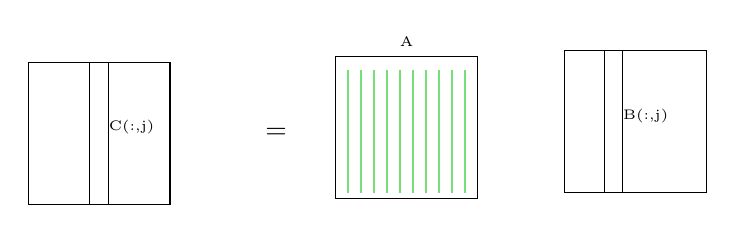
\begin{tikzpicture}[scale=1, every node/.style={transform shape}]
		%%	\tikzstyle{taskr}=[draw=black, minimum height=18mm, minimum width=18mm, anchor=south west, fill=pastelgreen, text=black]
		
		\tikzstyle{taskr}=[draw=black, minimum height=18mm, minimum width=18mm, fill=pastelgreen, text=black]
		
		\tikzstyle{taskrow}=[draw=black, minimum height=2mm, minimum width=18mm, fill=pastelgreen, fill=none, text=black]
		\tikzstyle{taskcol}=[draw=black, minimum height=18mm, minimum width=2mm, fill=pastelgreen, fill=none, text=black]
		
		\tikzstyle{taskrsmall}=[draw=black, minimum height=2mm, minimum width=2mm, fill=none, text=black]
		
		%%	\node(t1) at (0,0) {};
		%%	\node [above right=0cm and 0cm of t1.mid,taskr](T1) {};
		\node [taskr, fill=none] (T1) at (0,0) {};
		\node [taskcol] (T2) at (0,0) {};
		\node [right] at (T2.mid) {\tiny C(:,j)};
		
		\node[draw=none, text=black, scale=1] at (2.25,0) {$=$};
		%%	
		\node [right=3cm of T1.mid,taskr, fill=none](T3) {};
		%%	\node[taskrow](T4) at (T3.mid) {};
		\node [above] at (T3.north) {\tiny A};
		%%	\draw[pastelgreen, thick] (3.1cm, 0.8) -- (3.1cm, -0.75);
		%%	\draw[pastelgreen, thick] (3.2cm, 0.8) -- (3.2cm, -0.75);
		%%	\draw[pastelgreen, thick] (3.3cm, 0.8) -- (3.3cm, -0.75);
		%%	\draw[pastelgreen, thick] (3.45cm, 0.8) -- (3.45cm, -0.75);
		\foreach \x in {1,2,3,4,5,6,7,8,9,10}
		\draw [pastelgreen, thick] (3+0.165* \x, 0.8) -- (3+0.165* \x, -0.75);
		%%  \foreach \y [count=\yi] in {0,...,3}  
		%%  \draw (\x\y)--(\x\yi) (\y\x)--(\yi\x) ;
		
		%%	
		\node [right=2cm of T3.mid,taskr, fill=none](T5) {};
		\node [right=2.5cm of T3.mid, taskcol](T6) {};
		\node [right] at (T6.mid) {\tiny B(:,j)};
		%%	
		\end{tikzpicture}
	\end{center}
\end{frame}

\begin{frame}{Matrix multiplication: linear combination of rows}
	\begin{itemize}
		\item A row of $C$ is obtained by linear combination of rows of $B$.
	\end{itemize}
	\begin{center}
		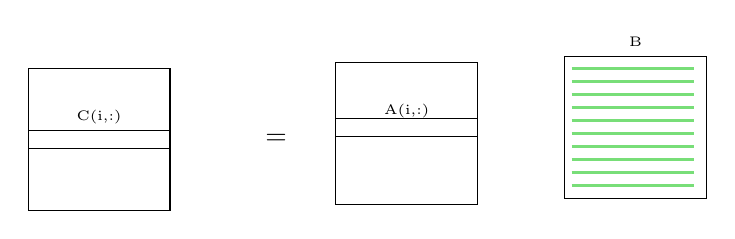
\begin{tikzpicture}[scale=1, every node/.style={transform shape}]
		%%	\tikzstyle{taskr}=[draw=black, minimum height=18mm, minimum width=18mm, anchor=south west, fill=pastelgreen, text=black]
		
		\tikzstyle{taskr}=[draw=black, minimum height=18mm, minimum width=18mm, fill=pastelgreen, text=black]
		
		\tikzstyle{taskrow}=[draw=black, minimum height=2mm, minimum width=18mm, fill=pastelgreen, fill=none, text=black]
		\tikzstyle{taskcol}=[draw=black, minimum height=18mm, minimum width=2mm, fill=pastelgreen, fill=none, text=black]
		
		\tikzstyle{taskrsmall}=[draw=black, minimum height=2mm, minimum width=2mm, fill=none, text=black]
		
		%%	\node(t1) at (0,0) {};
		%%	\node [above right=0cm and 0cm of t1.mid,taskr](T1) {};
		\node [taskr, fill=none] (T1) at (0,0) {};
		\node [taskrow] (T2) at (0,0) {};
		\node [above] at (T2.mid) {\tiny C(i,:)};
		
		\node[draw=none, text=black, scale=1] at (2.25,0) {$=$};
		%%	
		\node [right=3cm of T1.mid,taskr, fill=none](T3) {};
		\node[taskrow](T4) at (T3.mid) {};
		\node [above] at (T3.mid) {\tiny A(i,:)};
		%%	\node [above] at (T3.north) {\tiny A};
		%%	\draw[pastelgreen, thick] (3.1cm, 0.8) -- (3.1cm, -0.75);
		%%	\draw[pastelgreen, thick] (3.2cm, 0.8) -- (3.2cm, -0.75);
		%%	\draw[pastelgreen, thick] (3.3cm, 0.8) -- (3.3cm, -0.75);
		%%	\draw[pastelgreen, thick] (3.45cm, 0.8) -- (3.45cm, -0.75);
		%%	\foreach \x in {1,2,3,4,5,6,7,8,9,10}
		%%		\draw [pastelgreen, thick] (3+0.165* \x, 0.8) -- (3+0.165* \x, -0.75);
		%%  \foreach \y [count=\yi] in {0,...,3}  
		%%  \draw (\x\y)--(\x\yi) (\y\x)--(\yi\x) ;
		
		%%	
		\node [right=2cm of T3.mid,taskr, fill=none](T5) {};
		\node [above] at (T5.north) {\tiny B};
		
		\foreach \x in {1,2,3,4,5,6,7,8,9,10}
		\draw [pastelgreen, thick] (6, -0.75+0.165* \x) -- (7.56, -0.75+0.165* \x);
		
		%%	\node [right=2.5cm of T3.mid, taskcol](T6) {};
		%%	\node [right] at (T6.mid) {\tiny B(:,j)};
		%%	
		\end{tikzpicture}
	\end{center}
	
\end{frame}

\begin{frame}{Matrix multiplication: sum of $n$ matrices}
	\begin{itemize}
		\item Matrix multiplication can also be viewed as sum of $n$ matrices.
	\end{itemize}
	\begin{center}
		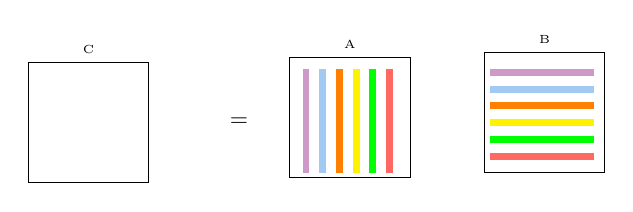
\begin{tikzpicture}[scale=0.85, every node/.style={transform shape}]
		%%	\tikzstyle{taskr}=[draw=black, minimum height=18mm, minimum width=18mm, anchor=south west, fill=pastelgreen, text=black]
		
		\tikzstyle{taskr}=[draw=black, minimum height=18mm, minimum width=18mm, fill=pastelgreen, text=black]
		
		\tikzstyle{taskrow}=[draw=black, minimum height=2mm, minimum width=18mm, fill=pastelgreen, fill=none, text=black]
		\tikzstyle{taskcol}=[draw=black, minimum height=18mm, minimum width=2mm, fill=pastelgreen, fill=none, text=black]
		
		\tikzstyle{taskrsmall}=[draw=black, minimum height=2mm, minimum width=2mm, fill=none, text=black]
		
		%%	\node(t1) at (0,0) {};
		%%	\node [above right=0cm and 0cm of t1.mid,taskr](T1) {};
		\node [taskr, fill=none] (T1) at (0,0) {};
		%%	\node [taskrow] (T2) at (0,0) {};
		\node [above] at (T1.north) {\tiny C};
		
		\node[draw=none, text=black, scale=1] at (2.25,0) {$=$};
		%%	
		\node [right=3cm of T1.mid,taskr, fill=none](T3) {};
		%%	\node[taskrow](T4) at (T3.mid) {};
		%%	\node [above] at (T3.mid) {\tiny A(i,:)};
		\node [above] at (T3.north) {\tiny A};
		%%	\draw[pastelgreen, thick] (3.1cm, 0.8) -- (3.1cm, -0.75);
		%%	\draw[pastelgreen, thick] (3.2cm, 0.8) -- (3.2cm, -0.75);
		%%	\draw[pastelgreen, thick] (3.3cm, 0.8) -- (3.3cm, -0.75);
		%%	\draw[pastelgreen, thick] (3.45cm, 0.8) -- (3.45cm, -0.75);´
		%%	  \foreach \x/\xtext in {0,...,3,2.72 / e} 
		\foreach \x/\y in {1/pastelviolet, 2/babyblueeyes, 3/orange, 4/yellow, 5/green, 6/pastelred}
		\draw [\y, line width = 2.5] (3+0.25* \x, 0.8) -- (3+0.25* \x, -0.75);
		%%  \foreach \y [count=\yi] in {0,...,3}  
		%%  \draw (\x\y)--(\x\yi) (\y\x)--(\yi\x) ;
		
		%%	
		\node [right=2cm of T3.mid,taskr, fill=none](T5) {};
		\node [above] at (T5.north) {\tiny B};
		
		\foreach \x/\y in {1/pastelviolet, 2/babyblueeyes, 3/orange, 4/yellow, 5/green, 6/pastelred}
		\draw [\y, line width = 2.5] (6, 1-0.25* \x) -- (7.56, 1-0.25* \x);
		
		%%	\node [right=2.5cm of T3.mid, taskcol](T6) {};
		%%	\node [right] at (T6.mid) {\tiny B(:,j)};
		%%	
		\end{tikzpicture}
	\end{center}
	
	\begin{center}
		
\begin{tikzpicture}[scale=0.85, every node/.style={transform shape}]
		%%	\tikzstyle{taskr}=[draw=black, minimum height=18mm, minimum width=18mm, anchor=south west, fill=pastelgreen, text=black]
		
		\tikzstyle{taskr}=[draw=black, minimum height=18mm, minimum width=18mm, fill=pastelgreen, text=black]
		
		
		%%	\node(t1) at (0,0) {};
		%%	\node [above right=0cm and 0cm of t1.mid,taskr](T1) {};
		\node [taskr, fill=none] (T1) at (0,0) {};
		%%	\node [taskrow] (T2) at (0,0) {};
		%%	\node [above] at (T1.north) {\tiny C};
		
		\node[draw=none, text=black] at (2.25,0) {$=$};
		
		\draw [pastelviolet, line width = 2.5] (3+0.25, 0.8) -- (3+0.25, -0.75);
		\draw [pastelviolet, line width = 2.5] (3+0.35, 1-0.25) -- (5, 1-0.25);
		\node[draw=none, text=black] at (5.25,0) {$+$};
		
		\draw [babyblueeyes, line width = 2.5] (2.5+3+0.25, 0.8) -- (2.5+3+0.25, -0.75);
		\draw [babyblueeyes, line width = 2.5] (2.5+3+0.35, 1-0.25) -- (2.5+5, 1-0.25);
		\node[draw=none, text=black] at (2.75+5.25,0) {$+\cdots$};
		
		\node[draw=none, text=black] at (3.5+5.25,0) {$+$};
		\draw [pastelred, line width = 2.5] (9.25, 0.8) -- (9.25, -0.75);
		\draw [pastelred, line width = 2.5] (9.35, 1-0.25) -- (9.35+1.65, 1-0.25);
		
		%%	
		%%	\node [right=3cm of T1.mid,taskr, fill=none](T3) {};
		%%	%%	\node[taskrow](T4) at (T3.mid) {};
		%%	%%	\node [above] at (T3.mid) {\tiny A(i,:)};
		%%	\node [above] at (T3.north) {\tiny A};
		%%	%%	\draw[pastelgreen, thick] (3.1cm, 0.8) -- (3.1cm, -0.75);
		%%	%%	\draw[pastelgreen, thick] (3.2cm, 0.8) -- (3.2cm, -0.75);
		%%	%%	\draw[pastelgreen, thick] (3.3cm, 0.8) -- (3.3cm, -0.75);
		%%	%%	\draw[pastelgreen, thick] (3.45cm, 0.8) -- (3.45cm, -0.75);´
		%%	%%	  \foreach \x/\xtext in {0,...,3,2.72 / e} 
		%%	\foreach \x/\y in {1/pastelviolet, 2/babyblueeyes, 3/orange, 4/yellow, 5/green, 6/pastelred}
		%%	\draw [\y, line width = 2.5] (3+0.25* \x, 0.8) -- (3+0.25* \x, -0.75);
		%%	%%  \foreach \y [count=\yi] in {0,...,3}  
		%%	%%  \draw (\x\y)--(\x\yi) (\y\x)--(\yi\x) ;
		%%	
		%%	%%	
		%%	\node [right=2cm of T3.mid,taskr, fill=none](T5) {};
		%%	\node [above] at (T5.north) {\tiny B};
		%%	
		%%	\foreach \x/\y in {1/pastelviolet, 2/babyblueeyes, 3/orange, 4/yellow, 5/green, 6/pastelred}
		%%	\draw [\y, line width = 2.5] (6, 1-0.25* \x) -- (7.56, 1-0.25* \x);
		%%	
		%%	%%	\node [right=2.5cm of T3.mid, taskcol](T6) {};
		%%	%%	\node [right] at (T6.mid) {\tiny B(:,j)};
		%%	%%	
		\end{tikzpicture}
	\end{center}
	
	
\end{frame}


\begin{frame}{Matrix multiplication: recursive calls on submatrices}
	\begin{itemize}
		\item Matrix is divided into 2$\times$2 blocks
	\end{itemize}
	%%\begin{pmatrix}
	%%	1 & 2 & 3\\
	%%	a & b & c
	%%\end{pmatrix}
	
	\begin{align*}
	\begin{pmatrix}
	C_{11} & C_{12} \\
	C_{21} & C_{22}
	\end{pmatrix}
	&
	=
	\begin{pmatrix}
	A_{11} & A_{12} \\
	A_{21} & A_{22}
	\end{pmatrix}
	\begin{pmatrix}
	B_{11} & B_{12} \\
	B_{21} & B_{22}
	\end{pmatrix}
	\end{align*}
	
	\begin{align*}
	C_{11} &= A_{11}B_{11} + A_{12}B_{21}\\
	C_{12} &= A_{11}B_{12} + A_{12}B_{22}\\
	C_{21} &= A_{21}B_{11} + A_{22}B_{21}\\
	C_{22} &= A_{21}B_{12} + A_{22}B_{22}\\
	\end{align*}
\end{frame}


\begin{frame}{Matrix multiplication: recursive calls on submatrices}
	Operation count recurrence,
	\begin{align*}
	T(n) &= 8T\Big(\frac{n}{2}\Big) + \mathcal{O}(n^2)\\
	T(n) &= 1
	\end{align*}
	Here $\mathcal{O}(n^2)$ refers that $\exists c\in\mathbb{N}$ such that this term is less than or equal to $cn^2$ for every $n$.
	\medskip
	
	
	After solving, we obtain $T(n) = \mathcal{O}(n^3)$.
\end{frame}


\subsection{Strassen's Matrix Multiplication}
	\begin{frame}{Table of Contents}		
	\tableofcontents[currentsection,currentsubsection] 		
	\end{frame}


\begin{frame}{Matrix multiplication: Strassen's algorithm}
	\begin{align*}
	\begin{pmatrix}
	C_{11} & C_{12} \\
	C_{21} & C_{22}
	\end{pmatrix}
	&
	=
	\begin{pmatrix}
	A_{11} & A_{12} \\
	A_{21} & A_{22}
	\end{pmatrix}
	\begin{pmatrix}
	B_{11} & B_{12} \\
	B_{21} & B_{22}
	\end{pmatrix}
	\end{align*}
	
	\begin{minipage}{0.45\columnwidth}
		\begin{align*}\small
		M_1 &= (A_{11} + A_{22})(B_{11}+B_{22})\\
		M_2 &= (A_{21} + A_{22})B_{11}\\
		M_3 &= A_{11} (B_{12}-B_{22})\\
		M_4 &= A_{22} (B_{21}-B_{11})\\
		M_5 &= (A_{11} +A_{12})B_{22}\\
		M_6 &= (A_{21}-A_{11})(B_{11} +B_{12})\\
		M_7 &= (A_{12}-A_{22})(B_{21} + B_{22}) 
		\end{align*}
	\end{minipage}
	\hfill
	\begin{minipage}{0.45\columnwidth}
		\begin{center}
			\begin{align*}
			C_{11} &= M_1 + M_4 -M_5 +M_7\\
			C_{12} &= M_3 + M_5\\
			C_{21} &= M_2 + M_4\\
			C_{22} &= M_1 -M_2 + M_3 + M_6
			\end{align*}
		\end{center}
	\end{minipage}
	
\end{frame}



\begin{frame}{Matrix multiplication: Strassen's algorithm}
	Operation count recurrence,
	\begin{align*}
	T(n) &= 7T\big(\frac{n}{2}\big) + \mathcal{O}(n^2)\\
	T(n) &= 1
	\end{align*}
	After solving, we obtain $T(n) = \mathcal{O}(n^{\log_2 7})$.\\
	$\qquad\qquad\qquad\qquad\qquad\log_2 7 \approx 2.81$
	%% \mathcal{O}(n^{2.81})$.
	\begin{block}{Open questions}
		\begin{itemize}
			\item Is there a way to perform matrix multiplication in less number of operations than this algorithm?
			\item What is the minimum number of operations to perform matrix multiplication?
		\end{itemize}
	\end{block}
\end{frame}
\section{Algorithms}
\begin{frame}
	\frametitle{Table of Contents}
	\tableofcontents[currentsection,hideallsubsections]
\end{frame}
\begin{frame}[fragile]{Analysis of traditional matrix multiplication algorithm}
	\begin{verbatim}
	//implements C=C+AB
	for i=1 to n
	for j=1 to n
	for k=1 to n
	C(i,j) = C(i,j) + A(i,k) * B(k,j);
	\end{verbatim}
	%%\only<2>{\begin{verbatim}
	%%	//implements C =C+AB
	%%	for i=1 to n
	%%	// read row i of A into fast memory  (total n read) 
	%%	for j=1 to n
	%%	// read row i of C into fast memory (total n read)
	%%	// read column j of B into fast memory (total n read)
	%%	for k=1 to n
	%%	  C(i,j) = C(i,j) + A(i,k) * B(k,j);
	%%	  // write row i of C back to slow memory (total n read)
	%%	\end{verbatim}
	%%$n^2 + 3n^2$ reads/writes combined dominates $2n^3$ computations}
\end{frame}

\begin{frame}[fragile]{Analysis of traditional matrix multiplication algorithm}
	\begin{verbatim}
	//implements C=C+AB
	for i=1 to n
	// read row i of A into fast memory  (total n*n reads) 
	for j=1 to n
	// read row i of C into fast memory (total n*n reads)
	// read column j of B into fast memory (total n*n*n reads)
	for k=1 to n
	C(i,j) = C(i,j) + A(i,k) * B(k,j);
	// write row i of C back to slow memory (total n*n writes)
	\end{verbatim}
	\medskip
	$n^3 + 3n^2$ reads/writes combined dominates $2n^3$ computations.
\end{frame}

\begin{frame}[fragile]{Tiled matrix multiplication}
	\begin{verbatim}
	//Consider, A, B, C to be n/b X n/b matrices of b X b subblocks
	//Asumme 3 bXb blocks fit in fast memory
	for i=1 to n/b
	for j=1 to n/b
	// read block C(i,j) into fast memory 
	// (total b*b*n/b*n/b = n*n reads)
	for k=1 to n/b
	// read block A(i,k) into fast memory 
	// (total b*b*n/b*n/b*n/b = n*n*n/b reads)
	// read block B(k,j) into fast memory 
	// (total b*b*n/b*n/b*n/b = n*n*n/b reads)
	C(i,j) = C(i,j) + A(i,k) * B(k,j); //Matrix multiplication in blocks
	// write block C(i,j) into fast memory 
	// (total b*b*n/b*n/b = n*n writes)
	\end{verbatim}
	\medskip
	$\frac{2n^3}{b} + 2n^2$ reads/writes $<<$ $2n^3$ computations.
\end{frame}

\begin{frame}{Amount of volume in matrix multiplication }
	\begin{itemize}
		\item Make b as large as possible, 3$b^2 \le M$
		\item Number of reads/writes $\ge 3^\frac{1}{2}n^3/M^\frac{1}{2} + 2n^2$
	\end{itemize}
	\vfill
	\brown{Question}: Is this optimal?

\end{frame}

\section{Communication bounds}

\end{document} 